\begin{figure}[h]
    \centering
    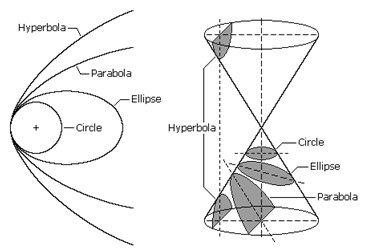
\includegraphics[scale=0.7]{AerospaceApplications/images/orb_dyn.png}
\end{figure}

After the explanation of the main topics about attitude kinematics, dynamics and control, we have to move to something also very important, but different.\\ We have said that a spacecraft can be thought as a rigid body and for this reason, its motion can be described separately in two parts: \textit{rotational motion} in which it is important to define the pshysical quantities in order to describe the attitude, then we study the \textbf{traslational motion} which include the study of the \textbf{orbital dynamics}, here how will be discussed, the presence of the gravitational field is very important.\\

Orbital dynamics is based on \textbf{celestial mechanics} which is composed by a set of equations:
\begin{itemize}
    \itemsep0em
    \item The three \textbf{Kepler's laws} which describe the motion of bodies on orbits in unperturbed system; 
    \item \textbf{Newton's laws} which are more general, moreover using them it is possible to derive the Newton's laws. They are three plus another which is the \textit{law of gravitation}.
\end{itemize}

\section{Fundamental laws}
\subsection{Kepler's laws}
\begin{enumerate}
    \item \textsf{\textbf{First} law}. A planet describes an \textbf{ellyptical orbit}, the sun is located in one of the foci; 
    \item \textsf{\textbf{Second} law}. The radius vector drawn from the sun to any planet sweeps out \textbf{equal areas in equal time}, that is the same to say that the \textbf{aeral velocity} is constant; 
    \item \textsf{\textbf{Third} law}. The \textbf{period of revolution} of a planet is proportional to $r_m^{3/2}$, where $r_m$ is the mean distance of the planet itself from the sun. 
\end{enumerate}

How we mentioned these laws are derived by using other general mechanics laws which are the three Newton's laws + law of gravitation.

\subsection{Newton's laws}
\begin{enumerate}
    \item \textsf{\textbf{First law}}. Unless an \textit{external force} acts, a particle remains at rest or continues to move at a \textbf{constant velocity}
    \footnote[1]{Note that when a particle remains at rest means that its velocity is such that $\mathbf{v}=0$, which is a \textbf{particular case} of constant velocity $\mathbf{v}=\text{const}$}; 
    \item \textsf{\textbf{Second law}}. The linear momentum {\footnote[2]{\textbf{Linear momentum} $\mathbf{p}=m\mathbf{v}$}} changes according to the following equation: 
    \begin{equation*}
        \frac{d}{dt}(m\mathbf{v}) = \textbf{F}
    \end{equation*}
    \begin{align*}
        &m: \quad \text{mass of the particle (could be varible in time)}\\
        &\mathbf{v}: \quad \text{velocity of the particle}\\
        &\mathbf{F}: \quad \text{Force acting on the particle (resultant)}
    \end{align*}
    \item \textsf{\textbf{Third law}} For any force $\mathbf{F}_{12}$ exerted by a particle 1 on a particle 2, there is a force $-\mathbf{F}_{21}$ from the particle 2 to the particle 1, on the same direction, opposite side.
    \item \textsf{\textbf{Law of gravitation}} Given two particles $m_1, m_2$, they attract \textbf{each other} with a force expressed as
    \begin{equation*}
        \mathbf{F} = G\frac{m_1m_2}{r^3}\mathbf{r}
    \end{equation*}
    \begin{align*}
        &m_1, m_2: \quad \text{particle masses}\\
        &\mathbf{r}: \quad  \text{vector of magnitude r which links the particles}\\
        &G: \quad \text{universal constant of gravitation}
    \end{align*}
\end{enumerate}

\section{The two-body problem}\footnote[3]{
    In the following the particle masses are assumed to be constant.
}
Putting together the basic notions we have presented, when you have two particles on which external forces are applied, an interesting problem arises which is the \textbf{two-body problem} on which for centuries scientists have dedicated their studies and efforts. It is extremely important when we are modeling the \textit{orbital dynamics} for aerospace applications, especially for a particular \textbf{restricted form}.\\
Let us consider two masses $m_1, m_2$ located in the positions $P_0$ and $P_1$ in an inertial frame {\footnote[4]{A reference frame with origin $O$ is said to be \textbf{inertial}, if $\dot{\mathbf{v}}=0 \iff \mathbf{v}=\text{const}$}} whose origin is $O$. It is useful to define the following quantities: 
\begin{itemize}
    \itemsep0em
    \item[\ding{202}] $\mathbf{r}_0, \mathbf{r}_1$ are the positions of the particle in the inertial reference frame, while their \textbf{relative position} is: $\mathbf{r}=\mathbf{r}_1-\mathbf{r}_0$;
    \item[\ding{203}]  $\mathbf{v}_0, \mathbf{v}_1$ are the velocities of the particle, equivalently to the positions, the quantity $\mathbf{v}=\mathbf{v}_1-\mathbf{v}_0$ is the \textbf{relative velocity}; 
    \item[\ding{204}] $\mathbf{F}_0$ and $\mathbf{F}_1$ are \textbf{external} (non gravitational) forces which are applied on the single particles.
    \item[\ding{205}] The \textbf{center of mass (CoM)} is characterized by the following quantities:
    \begin{itemize}
        \itemsep0em
        \item[\ding{52}] \textbf{CoM position}: it is the weighted mean of the single positions $$\mathbf{r}_c= \frac{m_0}{m_0+m_1} \mathbf{r}_0 + \frac{m_1}{m_0+m_1} \mathbf{r}_1$$ 
        \item[\ding{52}] \textbf{CoM velocity}: it is the weighted mean of the velocities
        $$
        \mathbf{v}_c = \frac{m_0}{m_0+m_1} \mathbf{v}_0+ \frac{m_1}{m_0+m_1} \mathbf{v}_1
        $$
    \end{itemize} 
\end{itemize}

Using these information, and doing some simple computation, a very important equation will be derived in the following.\\
By using the \textit{II Newton's law} we can write for each of the two bodies the equations: 
\begin{itemize}
    \item[\ding{202}] \textsf{\textbf{Particle $\mathsf{m_0}$}}. \begin{align*}
        m_0 \mathbf{v_0} = \sum{\mathbf{F}_i} &= G\frac{m_0m_1}{r^3}\mathbf{r} + \mathbf{F}_0 \overset{\frac{1}{m_0}}{\iff}\\
        &\mathbf{v_0} = G\frac{m_1}{r^3}\mathbf{r} + \frac{\mathbf{F}_0}{m_0}
    \end{align*}
    \item[\ding{203}] \textsf{\textbf{Particle $\mathsf{m_1}$}}.
    \begin{align*}
        m_1 \mathbf{v_1} = \sum{\mathbf{F}_i} &= -G\frac{m_0m_1}{r^3}\mathbf{r} + \mathbf{F}_0 \overset{\frac{1}{m_1}}{\iff}\\
        &\mathbf{v_1} =- G\frac{m_0}{r^3}\mathbf{r} + \frac{\mathbf{F}_1}{m_1}
    \end{align*}
\end{itemize}
Using the above equations we obtai, respectively, the expression for the \textit{relative velocity} and for the \textit{CoM velocity}.
\begin{align*}
    &\dot{\mathbf{v}}=\dot{\mathbf{v}_1} - \dot{\mathsf{v}_0} =- \frac{G(m_0+m_1)}{r^3}\mathbf{r} + \frac{1}{m_1} \biggl(
        \mathbf{F_1}-\frac{m_1}{m_0}\mathbf{F}_0 
    \biggr) \quad \textsf{(relative motion)}\\
    &\dot{\mathbf{v}}_c = \frac{1}{m_1} \frac{\mathbf{F}_1 + \mathbf{F}_0} {1+m_0/m_1} \quad \textsf{(CoM motion)}
\end{align*}
In some situations the particles $m_0, m_1$ have very different masses{\footnote[5]{ For instance: $m_0$: the Sun, $m_1$: the Earth, or $m_0$: the Earth, $m_1$: a satellite }} that is $m_0 \gg m_1$, then in the first equation above some terms are negligible. In particular, the first becomes:
\begin{equation} \tag{\textsf{2B}} \label{eq: 2B}
    \dot{\mathbf{v}} + \mu \frac{\mathbf{r}}{r^3} = \frac{1}{m_1} \mathbf{F}_1
\end{equation}
where $\mu=Gm_0$ is the \textit{gravitational parameter}. This important equation is called the \textbf{restricted two-body equation}{\footnote[6]{This is a nonlinear ordinary non-homogeneus differential equation, which has attracted the interest from the scientific community for centuries!}}.\\
When $m_0 \gg m_1$ holds, then $\mathbf{\dot{v}}_c=0$, this shows an interesting property: since the CoM has a constant velocity it can be choosen as the \textbf{origin of the inertial reference frame}. The next paragraph is dedicated to the  description of the properties of the equation (\ref{eq: 2B}).
 
\section{Free motion of the restricted two body problem}
It is interesting to study the \textbf{restricted two-body problem} derived from the fundamental laws in the particular case when \textbf{no external forces are applied}, to so-called \textbf{free motion}. The equation \ref{eq: 2B} becomes:
\begin{equation}\tag{\textsf{FR2B}} \label{eq: FR2B}
    \dot{\mathbf{v}} + \mu \frac{\mathbf{r}}{r^3}=0
\end{equation}
Starting from these equation important \textbf{conservation properties} are derived.

\subsection{Energy conservation}
If we make the dot product of the equation (\ref{eq: FR2B}) with $\mathbf{v}$ we obtain:
{\large{
    \begin{align*}
        &\dot{\mathbf{v}} \cdot \mathbf{v} + \mu \frac{\mathbf{r}}{r^3}\cdot \mathbf{v} =
        \frac{1}{2}\frac{d}{dt}(\mathbf{v}\cdot\mathbf{v}) + \frac{\mu}{2r^3}\frac{d}{dt}(\mathbf{r}\cdot\mathbf{r}) \underset{\frac{d}{dt}(r^2)=2r\frac{d}{dt}(r)=2r\cdot\dot{r}}{=}\\ 
        &\frac{d}{dt}\frac{v^2}{2} + \frac{\mu\dot{r}}{r^2} =\frac{d}{dt}\biggl(
            \frac{v^2}{2} - \frac{\mu}{r}
        \biggr) = \dot{\mathcal{E}}=0
    \end{align*}
}}
\noindent
We have proven that the physical quantity
\begin{equation*}
    \mathcal{E} = \frac{v^2}{2} - \frac{\mu}{r}
\end{equation*}
which is the \textbf{mechanical energy per unit mass}\footnote[7]{It is composed of two contributions: (i) \textbf{kinetic energy per unit of mass $\frac{v^2}{2}$}, (ii) \textbf{potential energy per unit of mass} $-\frac{\mu}{r}$ } is constant. For a given (total) energy $\mathcal{E}$ the orbital velocity is given by $v=\sqrt{2\mu/r+2\mathcal{E}}$

\subsection{Angular momentum conservation and planar motion}
Now let us the take the \textit{cross product} of the equation \ref{eq: FR2B} with $\mathbf{r}$ and we will obtain:
{\large{
    \begin{align*}
        &\mathbf{r} \times\dot{\mathbf{v}} + 
        \frac{\mu}{r^3}\mathbf{r} \times \mathbf{r} \overset{r\times r=0}{=} 
        \mathbf{r} \times\dot{\mathbf{v}} =\\
        & \mathbf{v} \times \mathbf{v} + \mathbf{r} \times\dot{\mathbf{v}} = \frac{d}{dt} (\mathbf{r} \times\mathbf{v})=0
    \end{align*}
}}
This proves that the quantity
\begin{equation*}
    \mathbf{h} = \mathbf{r} \times\mathbf{v}
\end{equation*}
the \textbf{angular momentum per unit of mass}, is constant since is derivative is null. Since $\mathbf{h}$ is the cross product between $\mathbf{r}$ and $\mathbf{v}$, it is orthogonal to the plane generated by $\mathbf{r}$ and $\mathbf{v}$, and since the angular momentum is constant, we have also proven that \textbf{the motion occurs on a plane} (which contains the orbit).

\subsection{Orbit equation (ORE)}
Let us take the cross product of the equation \ref{eq: FR2B} with the angular momentum $\mathbf{h}$ and we obtain the following result:
{\large{
    \begin{align*}
        \biggl(
            \dot{\mathbf{v}} +  \frac{\mu}{r^3}\mathbf{r}
        \biggr) \times \mathbf{h} = 
        \frac{d}{dt}\biggl(
            \mathbf{v} \times \mathbf{h} - \frac{\mu}{r}\mathbf{r}
        \biggr)=0
    \end{align*}
}}
The proof
\footnote[8]{Proof of the equality: \begin{align*}
    &\frac{d}{dt}(\mathbf{v}\times\mathbf{h}) = \dot{\mathbf{v}}\times\mathbf{h} + \mathbf{v} \times \dot{\mathbf{h}}= \mathbf{\dot{v}} \times \mathbf{h} \quad (\dot{\mathbf{h}}=0) \\
    &\frac{d}{dt}\biggl(
        -\frac{\mathbf{r}}{r}
    \biggr) = \frac{\dot{r}}{r^2} \mathbf{r} - \frac{1}{r}\mathbf{v} = \frac{1}{2r^3}\biggl(
        \frac{d}{dt} r^2
    \biggr) \mathbf{r} - \frac{1}{r}\mathbf{v} = \frac{1}{2r^3}\biggl(
        \frac{d}{dt} (\mathbf{r} \times \mathbf{r})
    \biggr) \mathbf{r} - \frac{1}{r}\mathbf{v}=\\
    &\frac{1}{r^3} ((\mathbf{r} \cdot \mathbf{v})\mathbf{r}-(\mathbf{r} \cdot \mathbf{v})\times \mathbf{v}=\frac{1}{r^3}\mathbf{r}\times(\mathbf{r}\times\mathbf{v}))=\frac{1}{r^3}\mathbf{r}\times\mathbf{h} \quad (\textsf{vector triple product})
\end{align*}}
of these first equality is based on simple manipulations which exploit some algebraic properties.
The above equation tells us that the quantity
$$
\mathbf{v} \times \mathbf{h} - \frac{\mu}{r}\mathbf{r}=\text{const} \doteq \mu\mathbf{e}
$$
where $\mathbf{e}$ is the \textit{eccentricity vector} and its norm $e=\vert \mathbf{e} \vert$ is called the \textit{eccentricity}. Let us take the dot product of r with the equation we have just derived:
\begin{align*}
    &\mathbf{r}\cdot (\mathbf{v} \times \mathbf{h}) - \frac{\mu}{r}\mathbf{r}\cdot\mathbf{r}=\mu\mathbf{r}\cdot\mathbf{e} \underset{\mathbf{r}\cdot (\mathbf{v} \times \mathbf{h})=(\mathbf{r}\times\mathbf{v})\cdot \mathbf{h}}{\iff} 
    (\mathbf{r}\times\mathbf{v})\cdot \mathbf{h} - \frac{\mu}{r}\mathbf{r}\cdot\mathbf{r}=\mu\mathbf{r}\cdot\mathbf{e}\iff\\
    &h^2 - \mu r = \mu \ r \ e \cos\theta \iff 
    h^2 = \mu \ r \ e \cos\theta + \mu r = \mu r(1+e \ \cos\theta)
\end{align*}
where $\theta$ is the angle between the relative position and the eccentricity vector and it is called the \textit{true anomaly}. By using this latest calculation, by expliciting the last step with respect to $r$ we obtain, given $p=h^2/\mu$ the so-called \textbf{semilatus rectum} or \textbf{parameter}:
{\large{
    \begin{equation} \tag{\textsf{ORE}} \label{eq:ORE}
        r = \frac{p}{1+e \cos\theta}
    \end{equation}
}}
this is the so-called \textbf{orbit equation}.


\section{Orbit geometry}
The equation (\ref{eq:ORE}) we have just seen is nothing but an equation of a conic section described in polar coordinates. We call \textbf{conic section} the curve obtained by intersect a cone with a plane with different angles of inclination.   \\
In the (\ref{eq:ORE}) equation the parameter which determines the shape is the \textbf{eccentricity}, in particular we obtain: 
\begin{itemize}
    \item An \textbf{ellipse} if $0 \le e < 1$, the ellipse collapses into a \textbf{circle} in the case that $e=0$, this is equivalent to state that a circle is a particular type of ellipse. Ellipses and circles are \textit{closed curves};
    \item A \textbf{parabola} if $e=1$, obtaining an \textit{open curve}; 
    \item An \textbf{hyperbola} if $e>1$, which is also an \textit{open curve}.
\end{itemize}
In the orbit equation other parameters appear which is the angle $\theta$ measured from the point nearest to the focus; $p$ (the parameter or semilatus rectum) determines the \textit{size} of the curve. \\
Once provided the general description of the conic sections, we can try to entry more into details of each type of curve.

\subsection{Ellipse}
\begin{figure}[h]
    \centering
    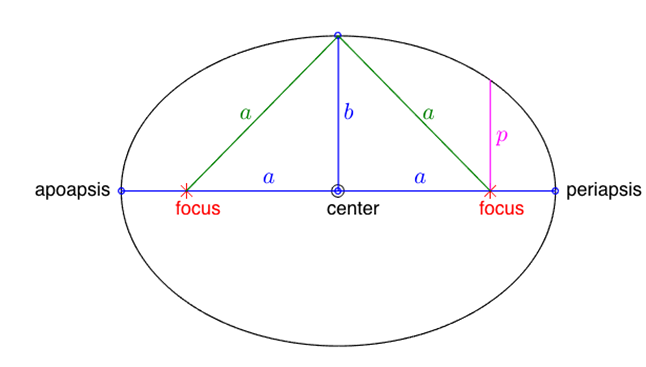
\includegraphics[scale=0.6]{AerospaceApplications/images/ellipse.png}
\end{figure}
\begin{quotation}
    \color{red}
    An \textbf{ellipse} is the locus of the point the sum of whose distances from two fixed points called \textbf{foci} is constant. 
\end{quotation}
The extreme point of the orbit are:
\begin{itemize}
    \item \textbf{Periapsis}: it is the point corresponding to $\theta=0$, in the case of motion around the Earth it is called \textbf{perigee}, on the other hand if the motion occurs around the Sun, it is called \textbf{perihelion}; the distance from the main focus is $r_p = p/(1+e)$
    \item \textbf{Apoapsis} it is the point correponding to $\theta=\pi$, it is called \textbf{apogee} or \textbf{aphelion}, if the motion occurs respectively around the Earth and around the Sun; here the distance from the main focus is $r_a = p/(1-e)$
\end{itemize}

Using the results of the mechanical fundamental law, of the gravitation law and the orbit equation we can derive the \textit{Kepler's law} we introduced in the first part of this  chapter.

\subsubsection{First law}
The \textbf{first Kepler's law} it is implied by the orbit equation if you put the eccentricity parameter $e$ such that $0 \le e < 1$.

\subsubsection{Second law}
The orbit area which is swept by the vector $\mathbf{r}$ in a time interval $\Delta t$ is equal to $\Delta A =\frac{1}{2}r (r\Delta \theta)$. Now, let us compute the derivative of $A$
\begin{equation*}
    \dot{A} = \lim_{\Delta t \to 0}\frac{\Delta A}{\Delta t} = 
    \lim_{\Delta t \to 0}\frac{r (r\Delta \theta)}{2\Delta t} = 
    \frac{r^2\dot{\theta}}{2} = \frac{h}{2} = \text{const}
\end{equation*}
Here we used the fact that the angular momentum is constant in presence of the (\ref{eq: FR2B}).

\subsubsection{Third law}
Let $A_p=\pi a b$ be the total orbital area and $P$ the period of the orbit, then 
\begin{equation*}
    P \equiv \frac{A_p}{A_p/P} = \frac{A_p}{\dot{A}}=
    \frac{2\pi a b}{h} = \frac{2\pi a^2 \sqrt{1-e^2}}{\sqrt{\mu a (1-e^2)}} = 2\pi \sqrt{\frac{a^3}{\mu}}
\end{equation*}
Since $\dot{A}$ is constant, then also the ratio $\frac{A_p}{P}$ is constant and equal to derivative itself.\\
For an elliptical orbit the energy $\mathcal{E}$ is negative.


\subsection{Parabola}
\begin{figure}[h]
    \centering
    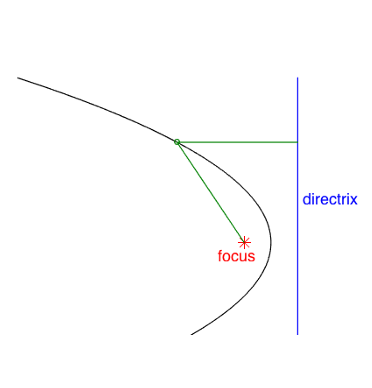
\includegraphics[scale=0.6]{AerospaceApplications/images/parabola.png}
\end{figure}

\begin{quotation}
    \color{red}
    A \textbf{parabola} is the locus of points whose distance from the focus is equal to the distance from a fixed line called the \textit{directrix}.
\end{quotation}
For a parabolic orbit the eccentricity is $e=1$, with a resulting null energy, that is $\mathcal{E} \to 0$.

\subsection{Hyperbola}
\begin{figure}[h]
    \centering
    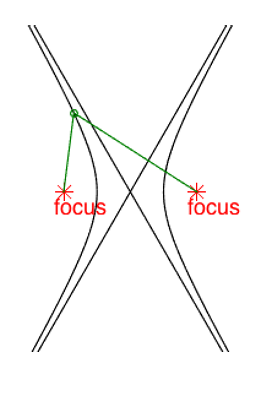
\includegraphics[scale=0.6]{AerospaceApplications/images/hyperbola.png}
\end{figure}
\begin{quotation}
    \color{red}
    An \textbf{hyperbola} is the locus of points the difference of whose from two fixed points called \textit{loci} is constant.
\end{quotation}
For an hyperbolic curve the eccentricity is $e>1$ with a resulting positive energy $\mathcal{E}>0$

\section{State equations}
For the \textit{orbital dynamics} the state equations are simply:
\begin{align*}
    &\dot{\mathbf{r}} = \mathbf{v}\\
    &\dot{\mathbf{v}} = -\frac{\mu}{r^3}\mathbf{r}
\end{align*}
Here the state variables are $\mathbf{x}=(\mathbf{r}, \mathbf{v})=(x_1, x_2, x_3, x_4, x_5)$, alternatively the state equations can be expressed in matrix form as: 
\begin{equation*}
    \begin{bmatrix}
        \dot{x_1}\\
        \dot{x_2}\\
        \dot{x_3}\\
        \dot{x_4}\\
        \dot{x_5}\\
        \dot{x_6}
    \end{bmatrix} = \begin{bmatrix}
        0&0&0&1&0&0\\
        0&0&0&0&1&0\\
        0&0&0&0&0&1\\
        -\frac{\mu}{r^3}&0&0&0&0&0\\
        0&-\frac{\mu}{r^3}&0&0&0&0\\
        0&0&-\frac{\mu}{r^3}&0&0&0
    \end{bmatrix}
    \begin{bmatrix}
        x_1\\
        x_2\\
        x_3\\
        x_4\\
        x_5\\
        x_6\\
    \end{bmatrix}
\end{equation*}

\section{Reference frames}
Elliptical and circular orbit are closed, moreover they are the trajectories of interest in the field of aerospace applications (spacecrafts, satellites, cubesats and so on). We can have several \textbf{reference frames} associated to an \textit{elliptic orbit}. In particular we will see:
\begin{itemize}
    \itemsep0em
    \item[\ding{202}] \textsf{\textbf{Local Vertical Local Horizontal frame (LVLH)}} (non inertial)
    \item[\ding{203}] \textsf{\textbf{Local Orbital Frame (LORF)}} (non inertial)
    \item[\ding{204}] \textsf{\color{red}\textbf{Perifocal (perigee) frame (PF)}} (inertial)
    \item[\ding{205}] \textsf{\color{red}\textbf{Geocentric equatorial frame (GF)}}. It is an \textit{inertial frame} associated with the Earth, it is very important especially in aerospace applications. 
\end{itemize}
As usual, a reference fram is made up of: (i) an origin, (ii) three unit vectors. For this reason in the next paragraphs the four proposed RF will be analysed specifying, for each one:
\begin{itemize}
    \itemsep0em
    \item Where is the origin;
    \item How the three unit vectors are defined.
\end{itemize}

\subsection{\textsf{\textbf{Local Vertical Local Horizontal frame (LVLH)}}}
\vspace{-0.5em}
\begin{figure}[h]
    \centering
    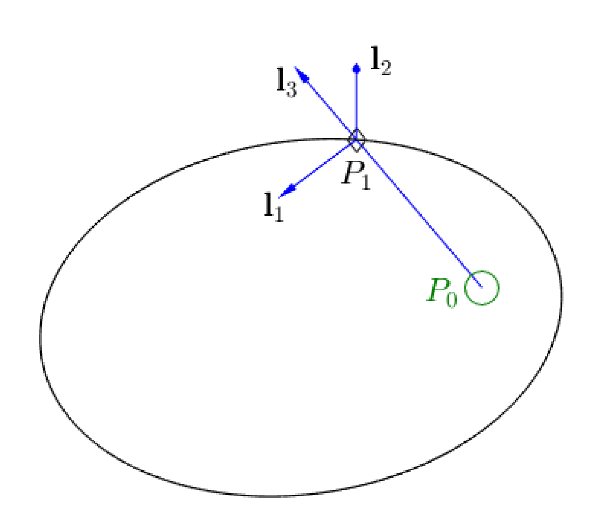
\includegraphics[scale=0.5]{AerospaceApplications/images/LVLH.png}
    \caption{Local Vertical Local Horizontal}
\end{figure}
\vspace{-1em}
{\Large\color{blue}
\begin{equation}
    R_l = \{
        P_1, \mathbf{l_1, l_2, l_3}
    \}
\end{equation}
}
The \textbf{origin} is at $P_1$ where the \textbf{smaller body} is located. The unit vectors:
\begin{enumerate}
    \item $\mathbf{l_3}$ is in the direction which links $P_1$ to $P_0$ (where the big body is located) this is called the \textbf{local vertical}; 
    \item Perpendicular to $\mathbf{l_3}$ you can find $\mathbf{l_1}$ which is \textbf{perpendicular} to $\mathbf{l_3}$ and in the orbital plane, the sign is the same with respect to the \textit{orbital velocity}; it is also called the \textbf{local horizontal}
    \item {\footnote[9]{
        This approach is used also for the other reference frames, and it is appropriate since the three unit vectors of a RF are \textbf{orthonormal} by definition.
    }}Having two out of three unit vectors, we can find the remaing one by doing the cross product $\mathbf{l_2} = \mathbf{l_3} \times \mathbf{l_1}$. It is called the \textbf{orbit pole}.
\end{enumerate} 
This is a \textbf{non inertial frame} because the origin, which is located in $P_1$ for sure does not have a constant velocity due to the fact its trajectory its a curve and at least the direction of the velocity (always tangent to the curve) \textbf{changes in time}.

\subsection{\textsf{\textbf{Local Orbital Frame (LORF)}}}
\vspace{-0.5em}
\begin{figure}[h]
    \centering
    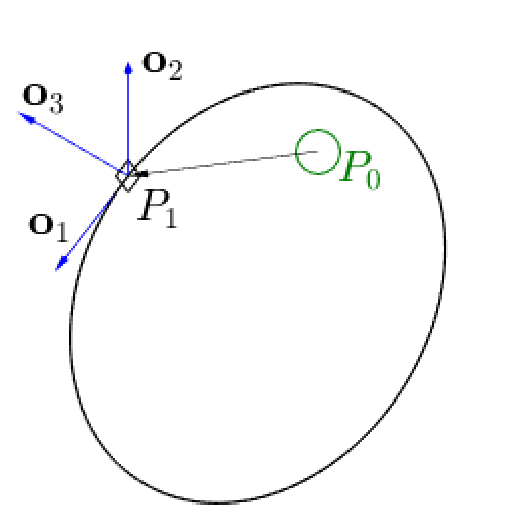
\includegraphics[scale=0.5]{AerospaceApplications/images/LORF.png}
    \caption{Local orbital frame}
\end{figure}
{\Large\color{blue}
\begin{equation}
    R_o = \{
        P_1, \mathbf{o_1, o_2, o_3}
    \}
\end{equation}
}
Here the \textbf{origin} is located in $P_1$ too, from this can be obtained that also in this case the reference frame in \textbf{non-inertial}. Reguarding the three unit vectors: 
\begin{enumerate}
    \itemsep0em
    \item $\mathbf{o_1}$ is obtained by the \textbf{instantaneous normalized velocity} and it is \textit{tangent} to the trajectory by construction; 
    \item $\mathbf{o_2}=\mathbf{l_2}$ is perpendicular to the orbital plane (also here it is called the \textbf{orbit pole}); 
    \item $\mathbf{o_3} =\mathbf{o_1} \times \mathbf{o_2}$ it is on the orbital plane. 
\end{enumerate}

\subsection{\textsf{\textbf{Perifocal (perigee) frame (PF)}}}
\begin{figure}[h]
    \centering
    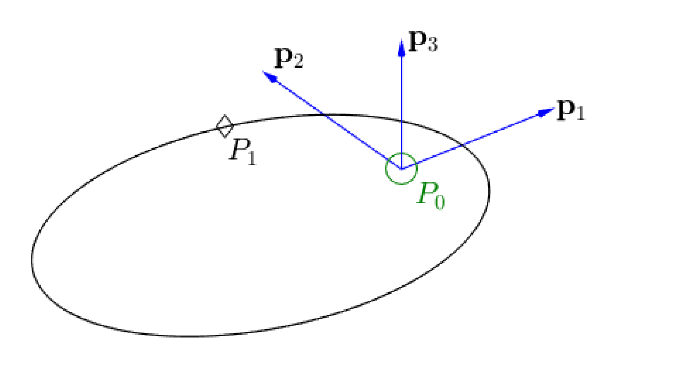
\includegraphics[scale=0.5]{AerospaceApplications/images/PF.png}
    \caption{Perifocal frame}
\end{figure}
{\Large\color{blue}
\begin{equation}
    R_p = \{
        P_0, \mathbf{p_1, p_2, p_3}
    \}
\end{equation}
}
Reguarding the \textbf{perifocal frame origin}, it is located at $P_0$ which is the position of the \textit{big body}. Neclecting its motion around the Sun, we can approximate this origin to be of constant velocity, determining an \textit{approximated} \textbf{inertial frame}. 
The \textbf{unit vectors} are defined as follows:
\begin{enumerate}
    \item $\mathbf{p_1=e}/e$ is the normalized eccentricity vectors which passes \textit{through the periapsis}, on  the orbital plane. 
    \item $\mathbf{p_3=o_2=l_2}$ is the orbit pole and again it is perpendicular to the orbital plane.
    \item $\mathbf{p_2 = p_3 \times p_1}$ is located on the orbit plane.
\end{enumerate}

\subsection{\textsf{\textbf{Geocentric equatorial frame (GF)}}}
\begin{figure}[h]
    \centering
    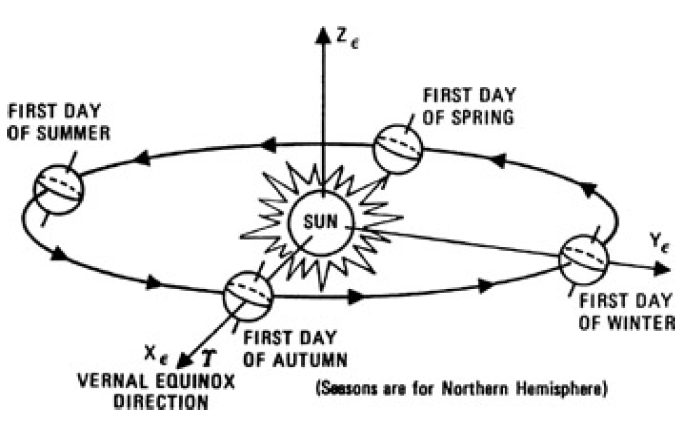
\includegraphics[scale=0.7]{AerospaceApplications/images/GF.png}
    \caption{Geocentric frame}
\end{figure}
\vspace{-0.8em}
{\Large\color{blue}
\begin{equation}
    R_{ge} = \{
        P_0, \mathbf{\hat{I}, \hat{J}, \hat{K}}
    \}
\end{equation}
}
This reference frame is used in the design of control systems for satellites, it is referred to the Earth and its definition is a little more complicated with respect to the others.\\
The \textbf{origin of GF} is at the \textbf{Earth CoM}, while the three unit vectors are defined as follows:
\begin{enumerate}
    \item $\mathbf{\hat{I}}$, in the direction \textsf{Earth $\to$ Sun} in the first day of spring (the so-called \textit{vernal equinox}).
    \item $\mathbf{\hat{J}}$ is obtained by computing the cross product between the others $\to$ $\mathbf{\hat{J} = \hat{K} \times \hat{I}}$
    \item $\mathbf{\hat{K}}$ is the \textit{polar rotation axis} and is orthogonal to the equatorial plane.
\end{enumerate}
It is a reference frame which is independent from the spacecraft orbit.

\section{Orbital elements}
\begin{figure}[h]
    \centering
    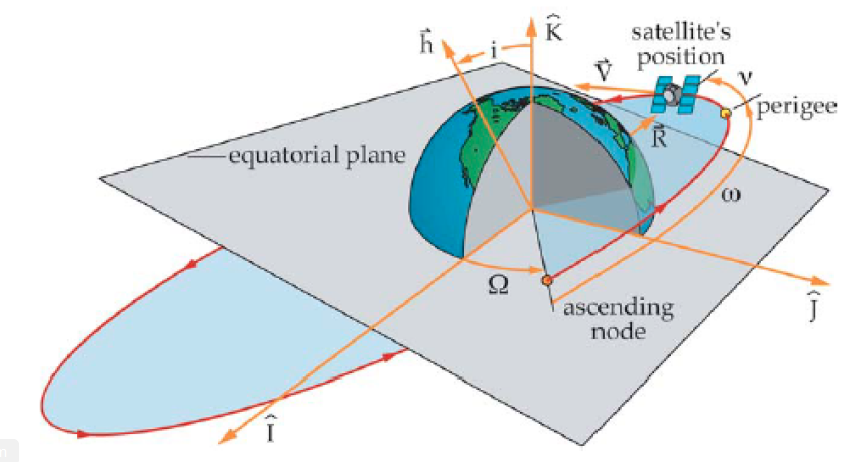
\includegraphics[scale=0.7]{AerospaceApplications/images/OrbElements.png}
\end{figure}
Let us focus our attention on \textbf{elliptic orbits} around the \textbf{Earth}. In this scenario \textbf{two different planes} can be individuated:
\begin{itemize}
    \itemsep0em
    \item The orbital plane
    \item The equatorial plane
\end{itemize}
The intersection between the two planes is called the \textbf{lines of nodes}{\footnote[10]{
    Remember that the intersection between two planes is a line.
}}, while the angle between the two planes normal direction is called \textbf{inclination} and is denoted with $i$.\\
The spacecraft orbit is a curve and its \textbf{intersection} with the equatorial plane is a point called \textbf{ascending node}. Other important angles can be defined:
\begin{itemize}
    \item The angle $\Omega$ is the argument of the ascending node on the equatorial plane, and it is the angle from $\mathbf{\hat{I}}$ to the \textit{ascending node}; 
    \item The angle $\omega$ is the angle from the ascending node to perigee (\textbf{on the orbilal plane});
    \item The angle $\nu$ o $\theta$ it is the \textbf{true anomaly} and it is the from the perigee to the \textit{spacecraft position}; sometimes instead of $\nu$ the \textit{time of perigee passage} $t_p$ is used, the two quantities are proportional.
\end{itemize}
We are ready the group together the \textbf{6 classical orbital elements}{
    \footnote[11]{
        \textit{classical} because in general you can define many orbital elements, however these are the most important.
    }
}. They are 
{\large{
    \begin{equation}
        (a, e, i, \Omega, \omega, \nu)
    \end{equation}
}}
where $a, e$ have been defined as the \textit{semimajor axis} and \textit{eccentricity} respectively. From the (\ref{eq: FR2B}) we know that the first five elements are constant and are related to the \textbf{orbit and its relative position wrt to the equatorial plane}, while $\nu$ changes in time and describe the position of the spacecraft on the orbit in time.\\
We have seen in the previous paragraph that we have \textbf{six state variables} related to $\mathbf{r}, \mathbf{v}$, it is possible to obtain starting from these the \textit{classical orbital elements}.\\
The following \textbf{coordinates transformation} holds:
{\large
\begin{itemize}
    \item \textsf{PF $\to$ GE}: $\mathbf{T}_{313}(\Omega,i,\omega)$; 
    \item \textsf{GE $\to$ PF}: $\mathbf{T}_{313}(-\omega, -i, -\Omega)$
\end{itemize}

}

\section{Orbit perturbations}
The orbital dynamics is based on \textbf{celestial mechanics} which is characterized by the Kepler's and Newton's laws. In order to simplify the discussion we have considered \textbf{(non-perturbed) Keplerian orbits} which are obtained by integration of the (\ref{eq: FR2B}), on the other hand \textbf{real orbits} are \textbf{non-Keplerian} in the sense there a lot of perturbations{\footnote[12]{
    In the sense that the term $(1/m_1) \mathbf{F}_1$ is not negligible and not null. 
}}: (i) the gravity potential due to a non-homogeneous distribution of the mass, (ii) interaction with other celestial bodies an so on.
Especially for \textit{LEO} an aerodynamic force has to be considered: the \textbf{drag force} of the atmosphere which is given by
\begin{equation}
    \mathbf{F}_d = -\frac{1}{2} \rho C_D S \vert \mathbf{v_{rel}} \vert \mathbf{v_{rel}}
\end{equation}
where:
\begin{itemize}
    \itemsep0em
    \item $\rho$ is the local atmospheric density defined as 
    \begin{equation*}
        \rho(r) = \rho_r \exp\biggl(
            -\frac{r-r_0}{H}
        \biggr)
    \end{equation*}
    with ($\rho_0, r_0$) the reference density and height, $H$ is a scale-height coefficient, while $r$ is the distance from the planet CoM.
    \item $C_D$ is the drag coefficient 
    \item $S$ is the area of the spacecraft directed in the direction of motion.
    \item While $\mathbf{v_{rel}}$ is the relative velocity of the spacecraft with respect to the atmosphere. Usually for simplicity $\mathbf{v}_{rel} \approx \mathbf{v}$ of the spacecraft.
\end{itemize}